\documentclass[sigconf, nonacm]{acmart}

\usepackage{booktabs} % For formal tables
\usepackage{lipsum}
\usepackage{csquotes}
\usepackage{subfigure}
\usepackage{listings}
\usepackage{xcolor}
\tolerance=100

% https://tex.stackexchange.com/questions/53941/verbatim-environment-with-background-color-pdflatex-and-tex4ht
\lstnewenvironment{code}{%
  \lstset{backgroundcolor=\color{lightgray},
  frame=single,
  framerule=0pt,
  basicstyle=\ttfamily,
  columns=fullflexible}}{}


\fancyhead{}

\title{The Development of a Web-based Multidimensional Data Plotter}
\subtitle{AC40001 Honours Project}


\begin{document}
\title{The Development of a Web-based Multidimensional Data Plotter}
\subtitle{AC40001 Honours Project}



\author{Sameer Al Harbi}
\author[0]{ID: 190007048/1}
\author[1]{BSc (Hons) Computing Science}
\author[2]{Supervisor: Dr. Iain Martin}
\affiliation{%
  \institution{University of Dundee}
  \city{Dundee}
  \country{UK}
}
\date{}


% The default list of authors is too long for headers.


\begin{abstract}
  This \textbf{should} be a \textit{summary} of ~250 words that summarises your project, including your aims and contributions that will arise from it. Think of it as a summary of your introduction.
\end{abstract}
\maketitle

\section{Introduction}


Data visualization is an important step in the data analysis process. Whether used on it's own as a tool for analysis, or as a final stop to clearly articulate and display results. It is in spirit a tool for communication, allowing abstract and complex ideas to be easily communicated to a wide audience, usually requiring minimal expertise to understand (Based on the visualization design done). It's ubiquity across all industries is then no surprise \cite{olshannikova_2015_visualizing}. Yet limitations and shortcomings exist, the accessibility of tools to create visualizations are often complex and at odds with the accessibility of the created artifacts. This limits creators by requiring them to have considerable knowledge of programming fundamentals, or be limited by what they are able to create. This is further compounded with 3D+ Multidimensional data visualization, Which has an even smaller selection of accessible tools.

Another challenge, when considering all tools regardless of user accessibility, has been the effect of Big Data on the user requirements of these applications. The ever increasing size and complexity of datasets doesn't invalidate the value provided by visualization to smaller datasets. In fact, It's importance as a communication aid is greater than ever before. Yet, current visualization tools and techniques cannot keep up with this requirement \cite{7918044}. In a way, this is just another accessibility problem- an inaccessibility of certain data types.

The aim of this project then was try to address the roots of these inaccessibility problems by creating a new market contender application focused with this problem in mind. This consisted of an academic long software development project undertaken by the student- with a resultant Multidimensional Scatterplot application created. This paper aims to highlight the decisions made in design and development while also recording the entire process followed by a look back on if the project was successful.










\section{Background}

The result of background research done for this project can be subdivided into two distinct sections being 'Related Work' and 'Tools and Technologies'. This was one of the earliest phases of the project whose results motivated the specific goals of this project- beyond just creating a Multidimensional plotting application as is required by the honours assessment that this project falls under, and explore what opportunities (in terms of tooling) exist to develop them.

\subsection{Related Work}
This section highlights the wider context that affected the structure and what the application was planned to do. The research identified here acted to directly influence what kind of application was developed, for what exact purpose and for what users.

\subsubsection{Project Context}
One of the first steps for this project was to place and understand the needs of this project through the lens of some wider context. By what metric should potential requirements be prioritised? and what those requirements should even be? Those are some of the questions whose answers will depend on the context that they are looked at. After some consideration, it was decided by the student to focus on the current business industry, and it’s needs as this context.

\begin{displayquote}
    This context (the business market) sets the aim of this project to then be an application that would be considered a valuable market entry compared to its competitors. It should also preferably, address some specific pain points of the market that are not fully covered by some other solution on the market.
\end{displayquote}

The alternative would also have been to look at this project from a more academic, literature driven view- where a project’s success would depend on more research oriented exploratory work. This alternative though, had some drawbacks that ultimately resulted in the selection of a Business Context. Mainly, a focus on existing market solutions allowed a more logical selection of features to develop for a practical development project. Although it should be stressed that this doesn’t mean that the academic background for this project was disregarded (See \ref{academicbackground})- It’s just that the focus was on the business-based requirements first and foremost.

\subsubsection{Market Research} \label{marketresearch}

With the context set- It was then considered that an analysis of the current options on the market would be a prudent next step to start understanding what a successful project should incorporate. This analysis was open-ended and focused on identifying key points that differentiated each product apart.

Detailed notes on each competitor can be found in the Appendix \ref{A1}, which are although not exhaustive, nevertheless highlight some important aspect of the overall market- But the main important trends and highlights identified are the following:

Firstly, it was found that most solutions are highly technical and need at least some degree of programming knowledge to use. A rough relationship would be that the complexity of using the solution and its capability is inversely proportional. Feature rich solutions need programming experience while the ones that don’t, have more limited features, and are more likely to be not free to use. Obviously, there were outliers such as MATLAB which have both a UI interface and a programming interface, but this relationship still stands.

Another interesting point identified is that The Stack Overflow 2021 Developer Survey \cite[]{stackoverflow_2021_stack} shows that a large majority of the most used libraries and frameworks were for data analysis or data-based projects, using specifically Python. Which is also the third most used language identified by the Survey \cite[]{stackoverflow_2021_stack}. Although these statistics don’t directly relate to visualization solutions, they help form an important background to the context in which visualization may be needed in. Which is that Python and its libraries are a highly prevalent option for undertaking data analysis projects, meaning that any visualization solution is likely to be part of a workflow that contains these tools.

But Solutions focusing on Visualization first and foremost seemed to be much fewer when compared to analysis solutions with visualization features. Those that were, were also much more likely to be highly technical. This point was found particularly important because data analysis and by extension visualization has been found to be needed in a wide field of industries, where programming expertise is not as widely common. And this need is expected to rise in the future with the advent of Industry 4.0- Which is a widely believed idea of increasing business productivity fueled by disruptive emergent technology in the near future \cite[]{GHOBAKHLOO2020119869}.

Taking all this into consideration, several key points were identified on how to structure a new development project to create a valuable solution from the market’s point of view:

\begin{itemize}
    \item Focus on accessibility first and foremost, including an easy-to-use interface that does not need programming experience.
    \item Focus on the visualization aspect, but either ensure that adequate analysis tools are available or importing or exporting data is easy and straight forward. Visualization is often only one step of a multi-step analysis project.
\end{itemize}

On the other hand, some thing’s to avoid are:

\begin{itemize}
    \item Focusing on the features but not accessibility. It is unreasonable to try to beat the current market players on features alone. You can’t get more feature-rich than a programming language such as Python, which is arguably one of the most used solutions on the market, See Appendix \ref{A1} for more information. It is important instead to create an alternative that is powerful enough but makes the process of data visualization much easier.
\end{itemize}

\subsubsection{Academic Background} \label{academicbackground}
A General study of research in the field was conducted with a focus on identifying any other similar projects such as this one undertaken by the student, and more importantly the wider context from an academic point of view. Which was followed by a comparison to previous market research in \ref{marketresearch}. This was done to give the student a better understanding of how visualization works in different settings and if there are any trends and patterns that can help prioritize functionality or uncover new opportunities.

This study was done by analyzing a small subset of important, state of the art research papers talking about data analytics and visualization. Some of these papers focus on market research which were particularly important to expand upon the market research done by the student themselves. The most important points identified are mentioned below (Consider this a continuation of the market research / section \ref{marketresearch} points above):

\begin{itemize}
    \item Current visualization techniques are not capable of handling big data \cite[]{7918044}. New solutions are being created and investigated by both industry and academia. Strategies for creating new visualization systems that handle each of the troubling aspects of big data have been put forward in \cite[]{9523950}. This is a big point that this project could contribute to fixing.
    \item No matter how good a visualization is- if it cannot be understood its value is nullified. There currently exists a gap between what computation is capable of creating and what can be easily grasped by a user. Naturally, there exists opportunity in creating solutions to close this gap by taking into consideration human cognitive psychology. \cite{olshannikova_2015_visualizing} \cite{7918044} \cite{10.1007/978-3-030-44999-5_39}
    \item Solving the problems to visualization poised by big data would require the combination of current visualization solutions merged with new technologies. \cite[]{olshannikova_2015_visualizing}
\end{itemize}

\subsubsection{Other Research} \label{otherresearch}
Another important aspect of research that was done included a more technical look into general design points that could help drive the design of the application itself and how features are developed.

One specific aspect researched has been software planning methodologies. The student was aware of agile and waterfall techniques from their study but those techniques were usually applied in and made for multi-person teams, which naturally conflicted with the single-person structure of this project. Through this research, a technique called PSP \cite[]{493023} (Personal Software Process) was discovered. This is a methodology that allows a singular developer to apply a structured, continuously improving process to how they develop software. A further inspired process was also identified called PXP \cite[]{10.1145/1593105.1593127}, which was a fusion of Agile XP principles adapted to a single person team inspired by PSP.

Another notable finding in this phase, was an analysis of graphing and visualization techniques. In the \ref{marketresearch} Market Research phase a lot of different solutions with a large variety of graphing types were seen. An analysis of the most common ones seen, which also had some overlap with The seven basic tools of quality (A collection of seven charts that need minimal training to use \cite[]{ishikawa_1985_what} for analysis) was undertaken with the hopes of identifying the most suitable graphs in terms of flexibility at higher dimensions (3+). The full analysis document can be seen in Appendix A2 but in summary- It was found that Scatterplot's fit these needs the most while also being part of the Seven tools meaning increased accessibility in who could use the application. The other main options included the Radar chart which was suitable but not part of the Seven tools.

\subsection{Tools and Technologies} \label{toolsntech}
Research was also done to highlight what technologies and design paradigms would be available for the development of this project. This also included a comparison between them. Though it should be noted that no decisions were made during this research stage of the project- The research and analysis recorded here act to justify and shortlist the final design in section \ref{techstack}

It should also be noted that obviously not all combinations of technologies mentioned below are viable. Usually deciding on one aspect would limit what can be selected for another. But nevertheless, each section below was looked at separately to fully understand the opportunity cost for each decision when going one route as opposed to another.

\subsubsection{Application Infastructure}
This section specifically focuses on the structural decisions in the design of an application that directly affect how it is created, run and in some cases what features are possible to implement. In general, the design options for this application in particular could be split into two groups.

\paragraph{Client-Side Run Application}
This is the simplest design. All code that makes up the application is run on the user’s device locally. No need for any server resources (Other than for serving the initial code which even then may not need a server, can distribute software on USB, Disc etc..) thus can be ran offline. But computing resources are limited to only what the user has and no inherit way to synchronize data among multiple users and devices- such as for user accounts, etc.

\paragraph{Server-Side or Full Stack Application}
This is a solution to some of the limitations mentioned for Client-side. Either have the client application be able to connect to a central (or server-less functions based) server and offload some tasks to it, or have the application be fully computed on-server with only static content responses being sent to the user. This design is naturally more complicated and often results in a split codebase among backend and frontend components. There is a need to provision computing resources, and more security considerations need to be made.

\subsubsection{Run Environment}
This can be defined as the software environment the application will run on and be thus designed for. The main options identified were the following:

\paragraph{.NET Environment}
.NET, which is an open-source developer platform for building Software supported by Microsoft \cite[]{microsoft_what}. It is cross platform among Windows, MacOS and Linux (With support for iOS and Android using frameworks such .NET Multi-platform App UI / MAUI \cite[]{davidbritch_what}). It provides a great rich set of libraries and tools for any kind of projects including both frontend and backend webapp needs and client ran applications (As long as .NET is installed on that device). .NET supports only 3 languages those being C\#, F\# and Visual Basic.

\paragraph{Node.js}
Node.js is aptly described on its website as an “an open-source, cross-platform JavaScript runtime environment.” \cite[]{nodejs_nodejs} It is the most popular web technology among the Stack Overflow 2022 Survey respondents \cite[]{stackoverflow_2021_stack}. Although most commonly used for Server-side processing as a webserver, it can also be used for running local applications as long as it is installed on the client’s device (although it usually makes more sense to serve the app over a network with node.js acting as a server side environment). For package managers, npm is tightly linked with node.js and provides a huge repository of packages. With the addition of Web Assembly, which is a new standard assembly like language that acts as a compilation target from a wide range of other languages, it is technically possible to use almost any language with node.js that has a compiler to web assembly made. \cite[]{webassembly}

\paragraph{Browser Engine}
Browser Engine’s- Modern browsers all have some JavaScript runtime engine, with V8 being the most widely used engine \cite[]{desktop} \cite[]{v8} Although all browsers are supposed to be cross-compatible, in practice this can vary, and some incompatibilities can arise. Browsers naturally only run client-side code but communicating with backend solutions is a common practice. Only JavaScript is natively supported and Web Assembly in “4 major browser engines”. \cite[]{webassembly}

\paragraph{JRE (Java Runtime Environment)}
JRE, is a runtime environment that allows an application to be cross compatible between Operating systems by acting as a compatibility layer. It runs Java bytecode which can be compiled from a large variety of languages. A standard library is also available with the runtime environment. Commonly used for backend development but also capable of Frontend.
\cite[]{amazon_what} \cite[]{oracle_what}

\paragraph{Compiled Program (OS only environment)}
Compiled Program, One of the most flexible options on the list. Languages such as C++ and C compile to machine code which are run directly on a user’s device. No inherit cross platform support and a need to recompile for each OS. Usually, higher performance due to lower abstraction. But a lower abstraction means more functionality needs to be managed by the programmer.

\subsubsection{Rendering Solution} \label{rendersol}
Being a project with visual requirements naturally meant that some rendering technology would be needed. Like with all other technologies mentioned thus far- there is a wide range of options that each have their own distinct design and ability. This section then aims to segment the available options by two factors at the minimum- One, the rendering solution must support 3D graphics in some capacity, and two, the solution must run and integrate with an application targeting one of the above-mentioned run environments. With those key requirements in mind, these were the identified options:

\paragraph{OpenGL}
OpenGL is a low-level cross-platform rendering API which can be traced back to a release date in 1992 \cite[]{wiki:opengl}. Although no longer in active development as of 2017, OpenGL still remains highly supported across both newly releasing GPUs and older. This also includes mobile devices. In terms of language bindings, OpenGL is cross-language and can be called from almost any language and environment that has had bindings made for it. \cite[]{segal_2022_the}

\paragraph{Vulkan}
Vulkan is a cross-platform low level open standard rendering API that has superseded OpenGL in active development by the Khronos Group, but does not replace it. It’s main driving improvement over OpenGL is lower overhead and more control over how code is run on the GPU. This greater control though does mean that development is more time consuming over OpenGL \cite[]{Vulkan}. Being much newer, with the initial release date being 2016 \cite[]{khronosgroup_2016_khronos}, it can be assumed to be much less supported among older devices than OpenGL.

\paragraph{Direct3D}
Direct3D is a subset API of the proprietary DirectX family of multimedia APIs developed by Microsoft \cite[]{grantmestrength_2021_direct3d}. It is a low-level API similar to OpenGL but created exclusively for Microsoft Windows, Xbox, and some Embedded Windows versions. In terms of languages, only C++ is supported targeting an executable on one of the above-mentioned systems \cite[]{stevewhims_2021_direct3d}.

\paragraph{WebGL}
A web integrated, JavaScript only low-level API version of OpenGL. It’s developed as an open web standard and is implemented in most widely used browsers, without the need to install it in any way for the client or developer. It’s a low-level API just like OpenGL and comes in two main versions based on OpenGL, WebGL 1.0 is based on the OpenGL ES 2.0 standard (OpenGL ES is an embedded subset version of OpenGL) while WebGL 2.0 is based on OpenGL ES 3.0 which is less supported among older devices. At the time of writing, WebGL remains the lowest level of abstraction for running GPU code on the web. \cite[]{mozilla_2019_webgl} \cite[]{khronosgroup_2011_webgl}

\paragraph{Metal}
Metal is a low-level rendering API designed by Apple for their devices. It has a very limited set of supported hardware and is further limited to only iOS and MacOS for the Operating System. In terms of language bindings; Objective-C, Swift and C++ are the only supported options. \cite[]{apple_metal} It was created by apple to replace OpenGL on their hardware which was depreciated in 2018. \cite[]{apple_apple}

\subsubsection{Optional Abstractions for Rendering Solutions}
The underlying rendering technologies mentioned in the last section, although usable on their own, can be offloaded to be managed by a higher-level framework or engine. Although it must be stressed that the inherit properties of the underlying rendering solution still has an effect on the application being developed.
The main reason to bring in an abstraction would usually be to lower development complexity, and in turn time. But the drawback often results in less flexibility regarding what can be made and lower performance.

\paragraph{Three.js}
Three.js is a JavaScript library that abstracts WebGL to simplify the creation of 3D graphics \cite[]{mrdoob_threejs}. It is highly extensive and offers a wide array of useful functions and constructs to that end. It is available as a npm package \cite[]{threejsorg_threejs} and can be easily integrated into a web-based project. If comparing to WebGL though, which is already a part of the browser, three.js contributes to a much bigger application download footprint. It also suffers from the same general relationship mentioned at the start of this section, development is greatly simplified but a lot of the flexibility and performance is lost.

\paragraph{Unity}
Unity, although first and foremost a game engine, can be applied to any development project where high performance graphics are needed. Unity supports DirectX, OpenGL, Vulkan and Metal- with only a few settings changes. A wide range of target devices can also then be built for. It is also possible to target WebGL as a platform in a similar fashion for web applications. Beyond this great cross-device and API support- Unity has an extensive collection of tools and APIs to streamline development. Although it should be mentioned that web applications are not as well supported, especially on mobile devices. The engine also only supports C\# as the only option. \cite[]{Nicoll2019} \cite[]{unitytechnologies_unity}

\subsubsection{Languages}
There are a large variety of potential languages that could be used for writing this program. The following were selected based on how extensively the languages are supported in previously mentioned Rendering solutions and Run Environment Sections. And some key exceptions that were considered to be important for consideration by the student.

\paragraph{C++}
A well know general-purpose compiled programming language most often used in performance critical applications. It is Object-Oriented but can be used to also write functional code. It is arguably the de-facto standard for systems programming. \cite[]{10.1145/323648.323736}

\paragraph{Rust}
Rust is a relatively new general-purpose compiled programming language often used in systems programming. It is a modern alternative to C++ that combines its high performance with a multitude of modern features such as a default package manager, and numerous safety features especially for memory (While still keeping a low performance impact). \cite[]{klabnik_2023_the}

\paragraph{Java}
Java is a general-purpose, object-oriented focused programming language that compiles to Java Bytecode that can be run on any device running a JVM (Java Virtual Machine). \cite[]{amazon_what} \cite[]{oracle_what}

\paragraph{C\#}
C\# is a general-purpose, multi-paradigm language developed by Microsoft. Although it is technically possible to compile to machine code, it is most often compiled to run on a .NET environment. \cite[]{B}

\paragraph{JavaScript}
JavaScript is the natively supported programming language on the web. It is multi-paradigm and is just-in-time compiled. It requires a runtime which is often a browser or dedicated runtime environments such as Node.js. \cite[]{mdncontributors_javascript}

\paragraph{TypeScript}
Typescript is a superset version of JavaScript developed by Microsoft with a number of features such as stricter syntax with the ability to have types. It transpiles to JavaScript which is then run in the same way. \cite[]{microsoft_typescript}

\subsubsection{Automated Testing}
Automated testing is used in software development to run a set of pre-configured tests repeatedly, usually every time before code is committed to a repository or as needed. Once tests are setup and written, it is an easy way to quickly test all cases including edge cases that would otherwise be tedious or take too long to do manually. Automated testing is not always possible for all aspects of an application but nevertheless a number of options were looked at in case an opportunity to integrate automated testing arises.

\paragraph{Test Complete}
Test complete is a GUI automation tool for testing a wide range of platforms and application types across Desktop, Web and Mobile platforms. \cite[]{smartbear_testcomplete}
But it's in-accessible price and no free tier limits it's adoptability for this project. \cite[]{smartbear_pricing}

\paragraph{Robot Framework}
Described on it's website as a "Robot Framework is a generic open source automation framework. It can be used for test automation and robotic process automation (RPA)." \cite[]{robotframework_robot} Being open-source it is free to use and has a wide range of libraries made for testing different device types and environments. \cite[]{robotframework_robot}

\paragraph{Selenium}
Selenium is a set of browser automation tools and libraries that can be applied to automate almost any part of browser interaction.
It is open source and free to use- It functions by providing a "WebDriver" interface for writing testing instructions that can be run on different browsers. Tests can be written
in a variety of languages but can only automate applications running in a browser. \cite[]{selenium_the}

\subsection{Summary} \label{ressummary}

The background research mentioned in this section acted to ground the other-wise open-ended project to a set of goals, both mandatory and optional, to create an impactful and original project. The following paragraph then summarizes the goals previously brought up into a short, guiding statement.

\begin{displayquote}
    The purpose of this project is to create a new market entry application for the creation of visualizations. This application would focus on user accessibility first and foremost, to be an application that is usable without programming knowledge. It will allow Multidimensional data to be plotted through a Scatterplot plot and possibly more chart options. In it's creation it will not ignore the current problems poised by Big Data and will attempt to support it thorough the application of state of the art techniques to support it's visualisations or be designed in such a way as to support their future integration into the application.
\end{displayquote}


Otherwise the research mentioned thus far also sets an origin from which all further decisions are justified by. For the final selection and analysis of the tech stack chosen by the student to develop the application, see section \ref{techstack}. To see how market research affected the application design, see section \ref{uxdesign}. These are just two of the bigger sections building upon the research set here- thus, other references linking here are to be expected as different parts of the project are focused on.



\section{Specification}
This section considers the formal project plan that was created for the development of this project, and the decisions on how it was structured. This phase of the project came after the specific project goals were identified during research (See \ref{ressummary}) and act's to create a development plan based on achieving these goals.

Each of the subsections then focus on one particular aspect of that planning.

\subsection{Development Methodology} \label{devmet}
PXP as introduced in the research phase \ref{otherresearch} was selected for its well defined (extensively documented) agile based methodology that was well suited to a single-person development team. Agile in general though, was selected over a waterfall technique to allow user feedback to drive design and development which was planned to be often collected.
As is a fundamental principle of agile this methodology was adapted to the project at hand (And the students work style) with some main changes and additions being:
\begin{itemize}
    \item Allow refactoring to be raised at any point, also allow grouping of similar user stories to be refactored together. Allow fixing problems before they became too big and interlinked.
    \item MoSCoW and Cost factors agile ceremonies were applied to the project’s user stories. Allowed better planning and time management.
    \item Instead of tasks created from user stories, user stories themselves were treated like tasks with any non-user story work labelled as tasks instead and treated the same as stories. Done to lower duplication of information and to fit better into GitHub Issues (See \ref{projectmanage})
    \item No automated testing. This was a decision that was retroactively added here after prototyping during the design phase (See \ref{automatedtests}). The justification for this change is covered there but in summary, It was found that Graphics development is fairly tricky to automate the testing of as the large majority of testing is completely visual and subject to changes.
    \item Reworked development process in general to better fit the students workflow. See \ref{scheduling} and \ref{devflow} for specific details
\end{itemize}

Feature sets were also adopted into the project. Where they played an important role in organizing tasks and user stories into logical sets based on source (User tester's suggestions, etc.) that could be prioritized and scheduled as part of a big picture overview. This big picture overview based on feature sets allowed the student to better manage their time by planning further ahead while still remaining flexible with development.

To see the resultant development flow with these changes in action see Section \ref{implementation}.

\subsection{Requirements Gathering} \label{reqgat}
With the goals that the developed application needs to achieve set as per the research phase (See \ref{ressummary})- It was considered important to then take these goals and create a concrete plan on what exact requirements would contribute towards achieving those goals. To do that, two main ideas were identified by the student.

The first idea was to conduct interviews with individuals who commonly use visualization tools or do general data science work. This would provide key insight into what real users of visualization technology think is key for a successful application to have. These requirements would constitute the first phase of the project and set a strong start to either a waterfall type methodology or an agile project.
But there were a couple of downsides that cancelled out this idea at that time:
\begin{itemize}
    \item With no initial product to focus insight into actionable requirements- the interview process is more likely to return conflicting or infeasible requirements.
    \item It might be difficult to offer insight that is not generic for the same reasons. "Application should plot data" vs "Application should do it like this instead of like that". With the latter insight being much more valued.
    \item Time and access to experts is very valuable and needs extensive preparation. It is important to make the most of it, which the student didn’t feel like they could do at that time as per the points mentioned so far.
\end{itemize}

The next idea to identify requirements was one which was inspired by the development methodology chosen to be followed by the student in section \ref{devmet}, PXP, the methodology in question, describes the process for a developer to stand in for the client if the client is unavailable for planning. So, The student took on the role of the client to create a client brief using the insight gained during the research phase. This had a number of key advantages listed as follows:

\begin{itemize}
    \item Minimal Preparation and much faster compared to planning and hosting an interview.
    \item Can take advantage of previous research into market competitors to inspire requirements.
    \item With the "Client" also being the developer it is possible to keep stories focused and ensure they are not conflicting.
\end{itemize}

With this technique, a planning stage was ran and a requirements brief was created. This brief can be read in full in Appendix \ref{A3} but in short, creates a written source document describing the minimum simplest application that would need to be created. It was considered that only a minimal version of the application should be planned at the beginning with further requirements created in a more agile way through user testing and analysis by the student based on how the project was progressing.

But the main reason to have created this brief instead of just skipping to creating user stories directly was to have a consistent main source from where user stories were pulled from initially that was focused on meeting the goals set during the research phase (See \ref{ressummary}).

The stories (formal requirements) extracted from the brief formed the MVP (minimum viable product) feature set which was scheduled as further covered in section \ref{scheduling} to be completed on the 16th of January. The specific extracted user stories and their analysis follow as per Table. \ref{req1}

\begin{table*}[t]
    \begin{tabular}{ | l | l | l | }
        \hline
        ID & Title                                                                                                               & Estimate (Relative) \\
        \hline
        1  & As a User, I want to be able to import a dataset into the application to graph it in a 3 dimension scatterplot      & 3                   \\
        \hline
        2  & As a User, I want to be able to navigate around the generated graph in 3D space while having the axis stay accurate & 6                   \\
        \hline
        3  & As a User, I want to be able to view a scatterplot of data set against an axis with accurate scales                 & 5                   \\
        \hline
        5  & As a User, I want to move the 3D view of the scatterplot in 3D using on screen controls                             & 3                   \\
        \hline
        6  & As a User, I want to be able to zoom in and out of the 3D Scatterplot                                               & 10                  \\
        \hline
        7  & As a User, I want to be able to rotate the 3D Scatterplot around all 3D axis individually                           & 5                   \\
        \hline
        8  & As a User, I want the application to have easy to use on screen controls for interacting with the application       & 3                   \\
        \hline
        9  & As a User, I want to be able to access the application on landscape screens of different sizes                      & 2                   \\
        \hline
        10 & As a User, I want to be able to view instructions within the application on how to use the application              & 2                   \\
        \hline
        11 & As a User, I want all interactable parts of the Application to be visible at all times                              & 1                   \\
        \hline
    \end{tabular}
    \caption{Requirements Gathering \#1 User Stories, MVP Feature Set, To be completed by January 16th}
    \label{req1}
\end{table*}

\subsection{Project Management Tools} \label{projectmanage}
A number of tools and services were employed in the development process to allow the organization and techniques mentioned to be applied. Those consisted of the following:

\subsubsection{Git, Version Control}
A version control tool is an important tool for controlling and recording changes to a codebase.
Git specifically though was chosen due to the student having previous experience, and to allow GitHub to be used within the project for it's supporting tools (See \ref{github} and \ref{github2}).

\subsubsection{GitHub, Cloud Code Repositary} \label{github}
Github is a cloud host for git repositories with additional extensive tooling to support all aspects of a software development project. The student has had extensive experience with this platform thus it was chosen for this project to minimize learning downtime. Alternatives such as Bitbucket and GitLab also existed but did not offer any further advantages that the student considered worth the learning downtime.

\subsubsection{GitHub Issues and Projects, Organizing Backlog and managing stories} \label{github2}
GitHub also has integrated issues and project views for organizing and tracking stories. An alternative would not have been as tightly integrated with the code repository.

\subsection{Scheduling} \label{scheduling}
When a backlog of user stories is ready the next step is to combine similar stories into feature sets with a set deadline for their completion (As mentioned in \ref{reqgat}). Then each user story and task within is analyzed using two main techniques:
\begin{itemize}
    \item Estimate - Based on how long a story would likely take to implement relatively to other stories in the feature set
    \item MoSCoW - A prioritization technique based on how critical the story is to the application. Where a story is given one of four categories of importance being Must, Should, Could and Won't in order of priority. \cite{articleMoscow}
\end{itemize}
With this, a prioritized backlog is created that is split among the maximum iterations/sprints that fit into the feature set's time frame with a consideration for the students iteration velocity, with stories themselves being prioritized to an earlier sprint based on their MoSCoW value. This combination of analysis allowed the student to prioritize which sprint the story should go in (Using MoSCoW) and then ensure that not too much work was assigned in the sprint (Using estimate rating). On the off chance that there wasn't enough time to complete all stories and tasks, the student would have re-analyzed what stories and tasks could be dropped due to time constraints, taking into consideration both the Estimate and MoSCoW values.

It should be though noted that the MVP feature set was treated a little bit different. MoSCoW analysis was not applied as each story was a "Must" by virtue of the feature set. It was also not initially split among sprints as other future feature sets were (See section \ref{usertest1}) due to little information on what the students velocity is at the time (start of development).

The specifics of when each feature sets deadline was set and how it changed can be seen on a sprint by sprint basis in the implementation section (See \ref{implementation}), in the Evaluation section (See \ref{usertest1}) and in the Requirements Gathering section (See \ref{reqgat}) based on the exact feature set.

\subsection{Development Flow} \label{devflow}
\begin{figure}
    \centering
    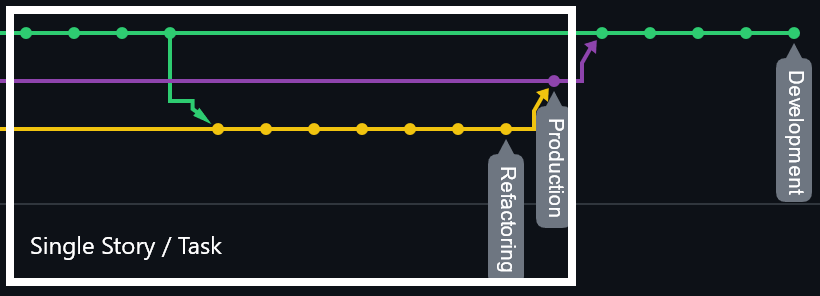
\includegraphics[width=1\columnwidth]{author-files/figures/SingleStoryPath2.png}
    \caption{Development Timeline of a Single Story}
    \label{fig:singlestory}
\end{figure}

Development followed a predefined process (See Figure \ref{fig:singlestory}) where a user story or task was picked to be developed from the prioritized backlog as per section \ref{scheduling}. Once the student has finished developing the one or more tasks/stories, the student would then push the code to the refactor branch where it would be organized and possibly reworked to follow better practices. This process allowed the student to move fast and encounter obstacles in implementation much more quickly, which minimized the risks of large roadblocks knocking the schedule out of balance. But once a feature/s was reworked to a sufficient standard with bugs fixed, it would then be fully tested and only then would be pushed to the final Production branch, which was build and publicly hosted.
This process helped ensure that any code committed to production was vetted and would be unlikely to cause unexpected issues. It also allowed the student to always have a safe version of the application for demos and user testing without having to worry about what work was done before hand.
The production version is then pushed to the development branch and the cycle repeats.



\section{Design}
An initial design phase was undergone by the student before development started. Although it should be noted that the work done did not constitute the final design as a waterfall methodology would require but was more akin to setting the scene for the start of development. The majority of design on how something should be coded, look and such was done on a story by story basis during sprints (See \ref{implementation})
This phase itself though consisted of the following key sections.

\subsection{Technology Stack} \label{techstack}
\begin{figure}[h]
    \centering
    
\includegraphics[width=1\columnwidth]{author-files/figures/logo-ts-webgl.PNG}
    \caption{TypeScript \cite[]{microsoft_2020_typescript} and WebGL logos \cite[]{khronosgroup_2017_the}}
    \label{fig:tswebgllogo}
\end{figure}
The student decided to settle on a technology stack during this phase. Which although would still be open to changes should they be needed if any problems arose during prototyping (See \ref{prototype}), nevertheless set what the stack should be otherwise. This decision was done by comparing valid options built up from those identified during the research phase (See \ref{toolsntech}) The selection and justification of every element of the stack follow below:

\paragraph{Client-Side run application}
This project was not expected to require any server resources such as central database access. As such, client-side only was chosen to allow the student to focus on a single code base. This also would simplify testing as there would be less infrastructure moving parts that could break.

\paragraph{Browser Run Enviroment}
Chosen for its greater accessibility over downloaded options and extensive support among devices without the need for any extra environment download by the user. Only a browser is needed which is usually preinstalled on most internet capable Operating Systems.

\paragraph{Rendering Solution}
WebGL, no other rendering API is as widely supported by major browsers that is capable of 3D graphics. WebGL1 is further picked as the target version to further increase compatibility.

\paragraph{Optional Abstractions for Rendering Solutions}
None, The student wanted to gain experience in how underlying low-level APIs worked, and did not want to sacrifice performance and flexibility of what was possible to create.

\paragraph{Languages}
With the browser set as the environment, the choice was limited to JavaScript, TypeScript or another language through Web Assembly. To ensure the best support among existent web tooling though, TypeScript was chosen which has the wide support of JavaScript while providing useful language features not available in JavaScript. One of those features, types, were found to be particularly important as OpenGL and by extension WebGL is very heavily dependant on correct types being used at all times, which would have been very hard to do with only JavaScript.

\subsection{Tooling}
After the Technology Stack was identified, the next step was to identify the development tools for that stack. The following were selected for the project:

\paragraph{IDE or Code Editor}
Visual Studio Code (VScode) was selected for all writing tasks (Both for code and writing latex). This decision came down to what the student was comfortable with using through previous experience but also had a practical factor for it's selection. With that mainly being a great selection of packages to help with development and great integration with GitHub.

\paragraph{Development Server}
Node.js was used as a development and build server due to it's straightforward ability to download and manage npm packages while also running development tools such as parcel, which in addition to it's usage below, also acted as a development server providing developer tools such as hot reloading on changes and helpful error screens.

\paragraph{Compiler and Build Tool}
As a compiler, Parcel was used to compile and optimize TypeScript into runnable by the browser JavaScript. As a build tool, parcel build all npm packages (including the usage of some node.js only features) into a handful of static client-side only files that could be hosted. This was crucial and allowed some code designs to be implemented that otherwise would not have been possible (See Model loading in \ref{prototype2}).

\paragraph{Hosting Provider}
Digital Ocean's App Platform was used to host and build the application from the production branch of the code repository. It was chosen due to the student having previous experience hosting resources on the platform, simple setup with minimal networking on the students part, integration with Github, support for building on a node.js environment (The same as the development environment, allowing for continuous integration from the production branch) and the availability of free credits to do all this. The site hosted here allowed user testers to access the application from anywhere at their own time.

\paragraph{Testing Framework} \label{testframe}
With this project set to run in a browser as per the rest of the technology stack (See \ref{techstack}). It was decided that Robot Framework would be the ideal choice for handling testing- This was expected to be done using WatchUI, a library for Robot Testing that runs selenium under the hood. This was done to make testing more flexible and less time consuming thanks to the wide selection of other helping libraries available with Robot Framework. Unfortunately, during prototyping (See \ref{prototype2}) a number of issues cropped up that ultimately left user testing to be set aside. For further details see \ref{automatedtests}.

\subsubsection{Additional Libraries}
The other mentioned npm packages used are recorded here and the reason for their use.

\paragraph{Pico.css}
Simple CSS framework to do the heavy lifting for styling the application UI. This allowed the student to focus more on rendering work.

\paragraph{gl-matrix}
Pre-made functions for the math very commonly used in graphics development. Allowed the student to bypass creating these basic functions from scratch in turn saving time.

\paragraph{jquery-csv}
A jquery syntax compliant .csv parser. No particular reason to select this particularly from other alternatives. Covers a lot of edge cases in parsing .csv files that would have taken a while to implement and test from scratch.

\subsection{Prototyping} \label{prototype}
An important part of the initial design stage was creating simple prototype applications using the technology stack to give the student experience with using the stack and to identify any critical issues that may need the stack to be redesigned or tools to be changed. These were in a sense mock sprint runs to smooth out the process and prepare for when development would officially start. The prototypes created also turned out general enough that they were able to be reused for the development of the actual application, in particular prototype 2.

\subsubsection {Prototype 1}
\begin{figure}[h]
    \centering
    
\includegraphics[width=1\columnwidth]{author-files/figures/tri.png}
    \caption{Prototype 1 - A simple 2D triangle drawn using the defined Technology Stack}
    \label{fig:prototype1}
\end{figure}

This was an important milestone in proving the validity of the development process identified. All of the tools and technologies mentioned thus far were setup and used to create a valid WebGL context and render a triangle (See Figure \ref{fig:prototype1}). It was found that this process was well defined and no changes were done.

\subsubsection {Prototype 2} \label{prototype2}
\begin{figure}[h]
    \centering
    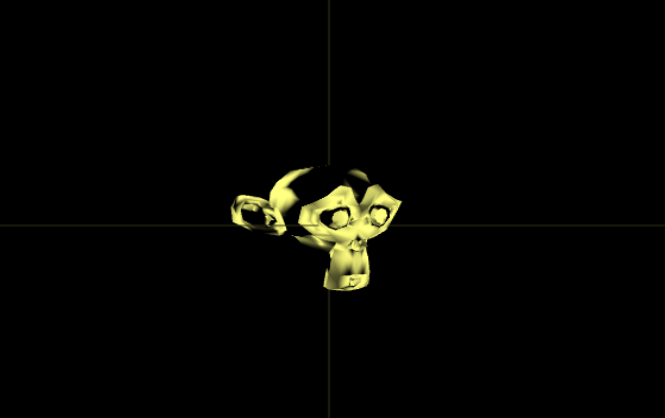
\includegraphics[width=1\columnwidth]{author-files/figures/Monkey-Test2.png}
    \caption{Prototype 2 - A 3D rendering engine}
    \label{fig:Monkey}
\end{figure}

\begin{figure}
    \centering
    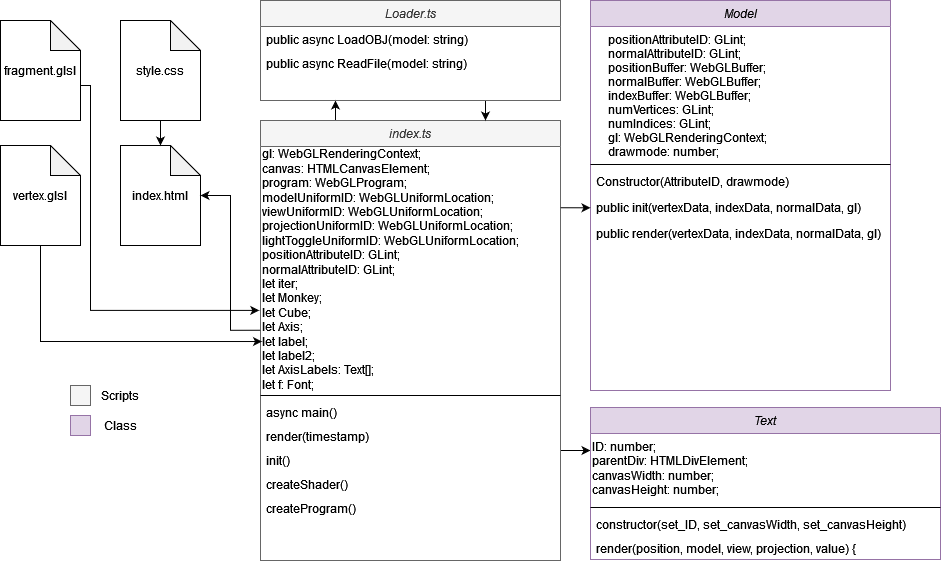
\includegraphics[width=1\columnwidth]{author-files/figures/UML_Prototype2fin.png}
    \caption{Prototype 2, Application Class Diagram}
    \label{fig:proto2class}
\end{figure}

\hfill

WebGL is a low level API and considerable work needs to be done just to render a 3D model. With this prototype, the aim was both to further test the tech stacks suitability by doing more involved work, but also to see if a general purpose rendering engine could be created that implemented all of the critical functions for the application to be developed. It was considered important to create this as quickly as possible to identify any shortcomings as soon as possible that may bottleneck the project when development starts. Creating this prototype took approximately a month and yielded in the creation of a successful rendering engine with a charting focused design.

To be more specific, the features implemented by this engine were the following:
\begin{itemize}
    \item 3D Mathematics with View, Projection and model system for rendering
    \item Multiple Models Rendered at the same time
    \item Model Object Abstraction for storing and rendering a 3D model. Implements a prototype pattern where one object can be rendered multiple times. This is particularly useful as a memory saving measure for rendering lot's of models. Something that was considered a very likely scenario for a plotting application with likely many data points.
    \item Simple Flat Shading based on a preset light direction.
    \item Loader Object for loading and organizing data that is passed to Model. Allows .OBJ models to be loaded into the renderer to be displayed. This used the node emulation feature provided by parcel to translate the written file system code to run in a browser, this meant files like .OBJ models and .glsl shader files could be kept separate from the renderer code and only combined when the application was built.
    \item Rendering labels with HTML and positioning them approximately at some relative to WebGL scene coordinates.
\end{itemize}

One bottleneck though was identified during this development, which was to do with Automated testing. See \ref{automatedtests} for the details.

\subsection{Testing Methodology} \label{automatedtests}
Test Driven development is an important aspect of the PXP process when developing software. This is most often done with automated testing for the best time efficiency and accuracy. But, during the creation of prototype 2 (See \ref{prototype2}) the student encountered a number of critical issues that contributed to the decision to not implement automated testing, subject to possible further consideration later on. Those issues were:

\begin{itemize}
    \item Graphics Development was found to be difficult to write tests for due to it's visual nature. This on it's own was not a problem as a solution using WatchUI was identified (See \ref{testframe}). What ended up being complex though was how rapidly the visuals changed during development, this made making tests useless as they could not be reused since they depended on comparing what the application rendered to reference images.
    \item Minimal UI to test, Automated testing on the web is particularly well suited to testing UI. Unfortunately, there wasn't any UI to test at the starting stages of development.
\end{itemize}

This points were expected to become less true as the application developed. Nevertheless, the student considered it unwise to setup tests for the start of development. Another process had to be identified in the meantime to allow the student to focus on bringing value to the project (completing user stories). This was the application of manual, visual inspection testing during the refactoring branch as per the specified development flow (See \ref{devflow}).


\begin{table*}[t]
    \begin{tabular}{ | l | l | }
        \hline
        Original                                             & Modified                                                    \\
        \hline
        Write chart properties programmatically              & Change properties through UI controls                       \\
        \hline
        Static chart image rendered once code written is run & Dynamically update rendered image as properties are changed \\
        \hline
        Difficult to explore                                 & Exploration possible                                        \\
        \hline
    \end{tabular}
    \caption{Comparison of design changes to how figures are created in the application developed compared to programmatic market alternatives}
    \label{compare}
\end{table*}

\subsection{UX Design} \label{uxdesign}

As mentioned in the research phase- Ease of use and accessibility for non-programmers was a priority for this project. One that had to also dictate design decisions around how a user would interact with the application and how that application would communicate with the user. Those key decisions are mentioned here.

\subsubsection{Visualisation Design} \label{visdesign}
One of the project's goals (See \ref{ressummary}) was to use a Scatter plot. To achieve that, two suitable rendering techniques were identified by the Student. Those are the following:

\begin{figure}[h]
    \centering
    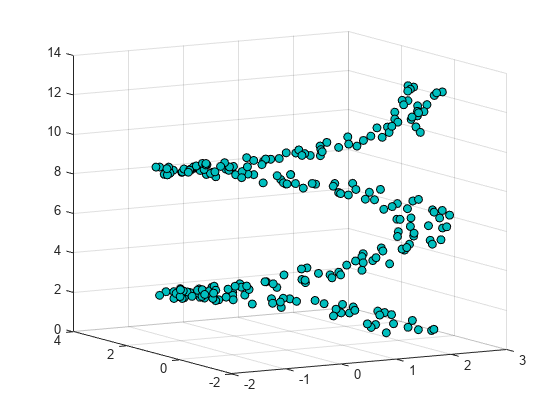
\includegraphics[width=0.7\columnwidth]{author-files/figures/SetMarkerPropertiesExample_01_MATLAB.png}
    \caption{A 3D scatterplot generated through MATLAB, example of a classic cut-off figure \cite{mathworks_3d}}
    \label{fig:MatlabPlot}
\end{figure}

\begin{figure}[h]
    \centering
    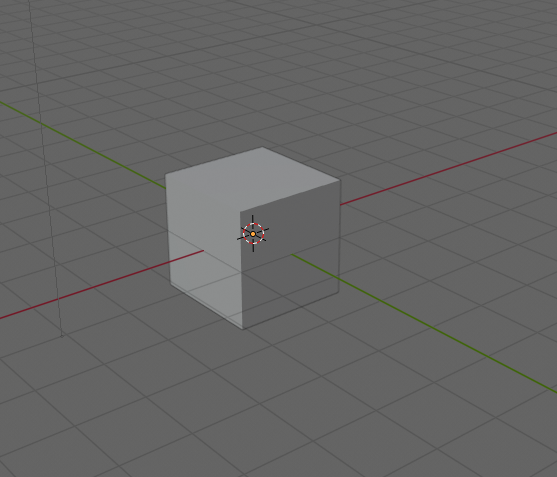
\includegraphics[width=0.7\columnwidth]{author-files/figures/worldnavblender.png}
    \caption{Screenshot from Blender \cite{blenderfoundation_2019_blenderorg}, A 3D modelling application, similar to the Unlimited Axis World view presented}
    \label{fig:blender}
\end{figure}

\begin{itemize}
    \item Unlimited Axis Values, World View. The scatterplot would be rendered into a 3D world by directly translating data values into world coordinates. The resultant graph could then be navigated by the user akin to 3D modelling software or a video game (first-person camera). Axis lines would be part of that world and would extend to infinity from origin. (See Figure \ref{fig:blender} for a visual example) This is a very easy to implement design but might be difficult to navigate for an inexperienced user and to appropriately combine together with UI across different screen sizes.
    \item Classic cut-off figure. This is directly inspired by the way the majority of applications seen implement scatterplots. As a user of those systems, you would load in some data and set aspects such as the position, view angle and zoom programmatically which would generate an image as seen in Figure \ref{fig:MatlabPlot}. This kind of view is not much harder to render but is much more concise as all data can be made to fit in a predefined visual space. This also allows greater control on how the graph is rendered allowing for a more consistent user experience to be tailored. But, this option has a severe disadvantage- where unlike the previous option, it is not commonly navigated but generated for specific parameters- making exploration not an obvious feature to implement.
\end{itemize}

In the end, the student decided to go with a modified option two. That modification was to replace the programmatic controls that have been seen to be used to compose / generate the chart in applications such as MATLAB (See Figure \ref{fig:MatlabPlot}) with instead corresponding UI controls. In a sense, the design that the student came up with abstracts the programming to user controls instead, which are much easier to use (which is the guiding goal for this project) even if they may be more limited in their capability. On input, the chart can be regenerated allowing exploration to be done in a similar sense, instead of moving the camera the chart is modified to show subsections of the data (See Table \ref{compare})

This would mean, as an example, instead of changing the view values in the code below and running the code again to look at the chart from a different angle: (Using code written in MATLAB \cite[]{mathworks_3d} to generate figure \ref{fig:MatlabPlot})
\begin{code}
    z = linspace(0,4*pi,250);
    x = 2*cos(z) + rand(1,250);
    y = 2*sin(z) + rand(1,250);

    scatter3(x,y,z,'filled')
    view(-30,10)
\end{code}
The user would be able to just click a button or drag their mouse to move the camera.

\subsubsection{User Controls}
The design created by the student in the last section (\ref{visdesign}) requires a robust design of user controls. The design and implementation for UI then followed an agile approach, where UI was designed and implemented as the need arose and the rendering counterpart could support it.

\subsection{Summary}
This design stage was critical in finalizing the last big questions that needed to be answered before development. With the application of the prototype phase (See \ref{prototype}), the student gained experience and confidence in working with the tools selected, meaning development could proceed much more smoothly.

\section{Implementation}
This project was developed over 8 sprints of between 7-10 days each with the first one started on the 26th of December, 2022 and the last one stared on March 19, 2023. What follows is a detailed summary of the work done during those sprints divided into three subsections:
\begin{itemize}
    \item Plan - Highlights what user stories were chosen to be implemented during the sprint and how long that sprint was.
    \item Implementation - How the features were implemented, any design decisions and any issues
    \item Summary - Have all user stories been completed? What went wrong? Anything learned and moved to next sprint
\end{itemize}

\subsection{Sprint 1 - Start 26th December}

\subsubsection{Plan}
This was the first sprint undertaken for the project and so the focus was to test everything out and ensure that the process was right for the student. The initial MVP feature set was chosen for development and two user stories were planned for. Those being user stories 3 and 11 with a total workload estimate of 6 over a 7 day sprint.
The main goal for this sprint was to create a labelled scatterplot graph with some pre-set test data.

\subsubsection{Implementation}
Prototype 2 was chosen to be extended into the application being developed. It was copied into the development branch and work started on implementing the user stories mentioned. A 3D Cube with axis lines was created as the chart and an origin position was set from which data points would be rendered. This was not as difficult as expected as the model matrix used could be copied and modified by each data point to ensure that they were always at a correct position relative to the cube and axis lines.

The next step was to label the axis lines (also relative to the chart using it's model matrix). This caused some difficulty as test labels would not align properly even if they were supposed to based on their coordinates. This was particularly troublesome with perspective lines that had a considerable z change in position. This was found to be a result of inaccurate placement by the browser (browsers favors flexibility over screen sizes instead of rigid pixel-perfect placement) and not fully correct world to screen coordinate calculation. Instead, it was decided that text should be rendered within the WebGL scene to ensure accuracy- To that end, a bitmap font technique was adopted.

\begin{figure}[h]
    \centering
    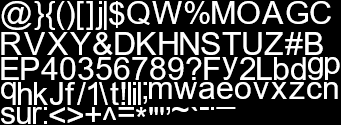
\includegraphics[width=0.5\columnwidth]{author-files/figures/glyphset.png}
    \caption{Arial font bitmap glyph image}
    \label{fig:arial}
\end{figure}

This is where a texture atlas with pre-rendered glyphs is downloaded and used to apply individual glyphs to flat surfaces (usually two triangles of geometry). This technique was mainly adopted due to it's simpler implementation and higher performance over the main alternative of using a geometric approach for rendering text (Where geometry is used to shape each glyph, which uses much more triangles). This alternative is highly inefficient as geometry is computationally expensive to render. Although it should be noted that bitmap font's do also carry their own limitations, mainly it is difficult to have large character sets as each character set would need to be saved into an image and downloaded, which if changing font sizes is required further requires that different sized copies of the character sets are available to avoid blurriness and pixelation at large sizes.
For this project though, those were considered to be tolerable limitations. Blurriness could be avoided by keeping glyphs the same size and the limited glyph set wouldn't matter as much with only one supported application language.
With bitmap fonts decided upon, the student started work on adapting the application to support rendering text in this way. This required a couple of key changes and additions within the renderer part of the application:
\begin{itemize}
    \item It should be possible to apply textures to models- This was done by adapting the Model class to store and apply texture data on render
    \item Textures had to rendered and stored- This was done by expanding the Loader class to allow .png images to be loaded
    \item There had to be some way to abstract which letter was rendered, manually slicing the bitmap texture to get each glyph would quickly become too tedious and time consuming for anything beyond a few glyphs- A State-Machine based Font Class was created that generated font texture data for an input letter that could be fed into a Model Object.
\end{itemize}

Have some class diagram here

\subsubsection{Summary}
The new technique for rendering text ended up fixing the accuracy issues caused by the previous label system and all user stories managed to be completed as expected and the application was pushed to production on january 1st, 2023. This was a slow start but the student expected that more user stories would be able to be tackled as they progressed with the project.

\subsection{Sprint 2 - Start 4th January}
\subsubsection{Plan}
This was the second sprint and the plan was to start adding user controls to allow a user to modify what was being rendered. This included not only the ability to upload custom data but also rotate the resultant graph. The MVP feature set was again the developed feature set from which 4 user stories were selected, with a total work load estimate of 16 over a longer 10 day sprint.


\bibliographystyle{ACM-Reference-Format}
\bibliography{bibliography}

\section{Appendices}
The following is a list of referenced appendices in the report. Please find the corresponding files in the submission.

\subsubsection{A1} \label{A1}
Notes on market competitors / similar applications on the market

\subsubsection{A2} \label{A2}
Analysis on different graph types and their application to 3D+ Data.

\subsubsection{A3} \label{A3}
Initial Requirements brief created by the student standing in for the Client.

\subsubsection{A4} \label{A4}
All testing datasets created for the project

\subsubsection{A5} \label{A5}
Latest HTML source code for testing instructions webpage, link to hosted page shared with testers and link to github repository

\subsubsection{A6} \label{A6}
User testing questionnaire questions and responses.

\subsubsection{A7} \label{A7}
Software source code, Latest Production branch

\subsubsection{A8} \label{A8}
Software source code, Production branch tested during User Testing 1

\subsubsection{A9} \label{A9}
Software source code, Prototype 2

\subsubsection{A10} \label{A10}
Software source code, Prototype 1

\subsubsection{A11} \label{A11}
User Manual, How to use the application and where to access it

\subsubsection{A12} \label{A12}
Meeting Minutes with advisor

\subsubsection{A13} \label{A13}
Ethics Declaration Form. Including the information sheet and a blank consent form.

\subsubsection{A14} \label{A14}
Risk Assessment Form

\subsubsection{A15} \label{A15}
Mid-term project progress report

\subsubsection{A16} \label{A16}
Project demonstrations material, includes a Poster

\subsubsection{A17} \label{A17}
UML diagrams

\end{document}